\section{Scope Graphs and Resolution Paths}
\sectionlabel{rescalc}

\lstset{language=PCFM}

Defining name resolution directly in terms of the abstract syntax tree leads to
complex scoping patterns.
In unary lexical binding patterns, such as lambda abstraction, the scope of the
bound variable is the subtree dominated by the binding construct.
However, in name binding patterns such as the sequential \pcfmcode{let} in ML,
or the variable declarations in a block in Java, the set of abstract
syntax tree locations where the bindings are visible does not necessarily 
form a contiguous region.
Similarly, the list of
declarations of formal parameters of a function is contained in a subtree of the
function definition that does not dominate their use positions.
Informally, we can understand these name binding patterns by a conceptual 
mapping from the abstract
syntax tree to an underlying pattern of \emph{scopes}.
However, this mapping is not made explicit in conventional descriptions of
programming languages.

We introduce the language-independent concept of a \emph{scope graph} to capture
the scoping patterns in programs.
A scope graph is obtained by a language-specific mapping from the abstract
syntax tree of a program.
The mapping collapses all abstract syntax tree nodes that behave uniformly with
respect to name resolution into a single `scope' node in the scope graph.
In this paper, we do not discuss how to specify such mappings for arbitrary
languages, which is the task of a binding specification language, but
we show how it can be done for a particular toy language, first by example and
then systematically. 
We assume that it should be possible to build a scope graph in a single
traversal of the abstract syntax tree.
Furthermore, the mapping should be \emph{syntactic}; \emph{no name resolution}
should be necessary to construct the mapping.  
%APT: repeats from intro.
%In previous work \cite{KonatKWV12} we have developed a generic name binding language,
%NaBL, that has these properties.
%The scope graph model developed in this paper is a generalization and formal
%definition of the resolution model underlying NaBL.

\begin{figure}[p]

\begin{minipage}[t]{.49\hsize}
\begin{boxedminipage}[t]{\hsize}
\textbf{References and declarations}
\begin{itemize}
  \item $\mbox{$\dsi{x}{i}{S}$}$: declaration with name $x$ at position $i$ and optional
  associated named scope $S$
  \item $\ri{x}{i}$: reference with name $x$ 
  at position~$i$ 
\end{itemize}
\textbf{Scope graph}
\begin{itemize}
  \item $\G$: scope graph
  \item $\S{\G}$: scopes $S$ in $\G$ 
  \item $\D{S}$: declarations $\dsi{x}{i}{S'}$ in $S$
  \item $\R{S}$: references $\ri{x}{i}$ in $S$
  \item $\I{S}$: imports $\ri{x}{i}$ in $S$
  \item $\P{S}$: parent scope of $S$
\end{itemize}
\textbf{Well-formedness properties}
\begin{itemize}
  \item $\P{S}$ is a partial function
  \item The parent relation is well-founded
  \item Each $\ri{x}{i}$ and $\di{x}{i}$ appears in exactly one scope $S$
\end{itemize}
\end{boxedminipage}
\caption{Scope graphs}
\figurelabel{scope-graph}
\end{minipage}
\begin{minipage}[t]{.49\hsize}
\begin{boxedminipage}[t]{\hsize}
\textbf{Resolution paths}
\vspace*{-0.4\baselineskip}
$$\begin{array}{rl}
          s & := \dstep{\di{x}{i}}\ |\ \istep{\ri{x}{i}}{\dsi{x}{j}{S}}\ |\ \pstep\\
          p & := []\ |\ s\ |\ p\cdot p\\
          & \mbox{\rm (inductively generated)} \\[0pt]
          [] \cdot p & = p \cdot [] = p\\
          (p_1 \cdot p_2) &\cdot\ p_3  = p_1 \cdot (p_2 \cdot p_3)
\end{array}$$ 

\textbf{Well-formed paths}

\vspace*{-0.5\baselineskip}

\[
	   \WF(p) \Leftrightarrow p \in \pstep^* \cdot \istep{\_}{\_}^* 
\]
	
\textbf{Specificity ordering on paths}

%\bigskip

	\infrule{DI}{}{
		\dstep{\_} < \istep{\_}{\_}
	}

\medskip

	\infrule{IP}{}{
		\istep{\_}{\_} < \pstep 
	}

\medskip

	\infrule{DP}{}{
		 \dstep{\_} < \pstep
	}

\medskip

    \infrule{Lex1}{
		s_1 < s_2
	}{ 
		s_1\cdot p_1 < s_2 \cdot p_2
	}


\medskip

	\infrule{Lex2}{
		p_1 < p_2
	}{ 
		s \cdot p_1 < s \cdot p_2
	}

\smallskip

\end{boxedminipage}
\caption{Resolution paths, well-formedness predicate, and specificity
ordering.}
\figurelabel{order}
\end{minipage}

\bigskip

\begin{boxedminipage}{\hsize}
\textbf{Edges in scope graph}
\smallskip

	\infrule{P}{
		\P{S_1} = S_2
	}{
		\seeni \vdash \pstep : S_1 \edge S_2
	}

\medskip

	\infrule{I}{
		\ri{y}{i} \in \I{S_1}\setminus\seeni  
		\tab
		\seeni \vdash p : \ri{y}{i} \resolve \dsi{y}{j}{S_2}
	}{
		\seeni \vdash \istep{\ri{y}{i}}{\dsi{y}{j}{S_2}} : S_1 \edge S_2 
	}

\medskip
\textbf{Transitive closure}

%\medskip
       
	\infrule{N}{
		}{
		\seeni \vdash [] : A \medge A
	}

\medskip

	\infrule{T}{
		\seeni \vdash s : A \edge B
		\tab 
		\seeni \vdash p : B \medge C
	}{
		\seeni \vdash s \cdot p : A \medge C
	}

\smallskip

\textbf{Reachable declarations}
\medskip

	\infrule{R}{
		\di{x}{i} \in \D{S'}
		\tab
		\seeni \vdash p : S \medge S'
		\tab 
		\WF(p)
	}{
		\seeni \vdash p \cdot \dstep{\di{x}{i}} : S \reach \di{x}{i}
	}

\medskip

\textbf{Visible declarations}
\medskip

\infrule{V}{
 	\seeni \vdash p : S \reach \di{x}{i}
			\tab
			\tab
			% tab
  		\forall j,p' (
  		   \seeni \vdash p' : S \reach \di{x}{j} \Rightarrow 
  		   \neg (p' < p)
  		)
  	}{
		\seeni \vdash {p} : S \resolve \di{x}{i}
	}

\medskip

\textbf{Reference resolution}

\medskip 

\infrule{X}{
		\ri{x}{i} \in \R{S}
    \tab
    \{ \ri{x}{i} \} \cup \seeni \vdash p : S \resolve \di{x}{j}
	}{
		\seeni \vdash p : \ri{x}{i} \resolve \di{x}{j}
	}
\end{boxedminipage}
\caption{Resolution calculus}
\figurelabel{rescalc}



\end{figure}



Figures \ref{fig:scope-graph} to \ref{fig:rescalc} define the full theory.
\Figure{scope-graph} defines the structure of scope graphs.
\Figure{order} defines the structure of \emph{resolution paths}, a subset of
resolution paths that are \emph{well-formed}, and a \emph{specificity ordering} on
resolution paths.
Finally, \Figure{rescalc} defines the \emph{resolution calculus}, which consists
of the definition of \emph{edges} between scopes in the scope graph and their
transitive closure, the definition of \emph{reachable} and \emph{visible}
declarations in a scope, and the \emph{resolution} of references to
declarations.
In the rest of this section we motivate and explain this theory.



\subsection{Example Language}

\begin{figure}[t]
\begin{boxedminipage}{\hsize}
\begin{grammar}
\sdnn{\pcfmcode{program}}{\ks{\w{\pcfmcode{decl}}}}
\\
\sdnn{\pcfmcode{decl}}{\text{\pcfmcodemm{module}}\ \w{\pcfmcode{id \{}}\ \ks{\w{\pcfmcode{decl}}}\ \kw{\pcfmcode{\}}}}
\altf{\text{\pcfmcodemm{import}}\ \w{\pcfmcode{qid}}}
\altf{\text{\pcfmcodemm{def}}\ \w{\pcfmcode{id}}\ \kw{=}\ \w{\pcfmcode{exp}}}
\\
\sdnn{\pcfmcode{exp}}{\w{\pcfmcode{qid}}}
%\altf{\kw{(}\ \w{exp}\ \w{)}}
%\altf{\kw{ifz}\ \w{exp}\ \kw{then}\ \w{exp}\ \kw{else}\ \w{exp}}
\altf{\text{\pcfmcodemm{fun}}\ \w{\pcfmcode{id \{ exp \}}}}
\altf{\text{\pcfmcodemm{fix}}\ \w{\pcfmcode{id \{ exp \}}}}
\altnn{\text{\pcfmcodemm{let}}\ \ks{\w{\pcfmcode{bind}}}\ \text{\pcfmcodemm{in}}\ \w{\pcfmcode{exp}}}
\altf{\text{\pcfmcodemm{letrec}}\ \ks{\w{\pcfmcode{bind}}}\ \text{\pcfmcodemm{in}}\ \w{\pcfmcode{exp}}}
\altf{\text{\pcfmcodemm{letpar}}\ \ks{\w{\pcfmcode{bind}}}\ \text{\pcfmcodemm{in}}\ \w{\pcfmcode{exp}}}
\altnn{\w{\pcfmcode{exp}}\ \w{\pcfmcode{exp}}}
\altf{\w{\pcfmcode{exp}}\ \kw{\oplus}\ \w{\pcfmcode{exp}}}
\altf{\w{\pcfmcode{int}}}
\\
\sdnn{\pcfmcode{qid}}{\w{\pcfmcode{id}}}
\altf{\w{\pcfmcode{id}}\ \kw{.}\ \w{\pcfmcode{qid}}}
\\
\sdnn{\pcfmcode{bind}}{\w{\pcfmcode{id}}\ \kw{=}\ \w{\pcfmcode{exp}}}
%\mc{id}{identifiers}
%\\
%\mc{int}{integer constants}
\end{grammar}
\end{boxedminipage}
\vspace*{-\baselineskip}
  \caption{Syntax of LM.}
  \figurelabel{pcfm:grammar}
\end{figure}
  

%\begin{figure}[t]
%\begin{boxedminipage}{\hsize}
\begin{lstlisting}
module A {      // module definition
  import B      // import of content of module
  import C      // import through import
  def a = 0      
  def b = a  
  def b = b + c // access imported definition
}
module B {
  module C {
    def c = D.f(3) // qualified access
  }
  module D {
    def f = 
      fix f {      // shadowing 
        fun n {    // m
          ifz n then 1 else n * (f (n - 1))
        } 
      }
  }
}
// todo: no def-before-use
// todo: transitive import
// todo: let binding
\end{lstlisting}
% module C {
%   import B
%   ...
% }
% module B {
%   import A
%   def x = 1
%   def x =2
% }
% module A {
%   def y = 5
% }
% module C {
%   import B
%   def z = x + y
% }
%\end{boxedminipage}
\caption{Example LM program.}
\figurelabel{example-program}
\end{figure}


To illustrate the scope graph framework we use the toy language LM, defined in
\Figure{pcfm:grammar}, which contains a 
rather eclectic combination of features chosen to 
exhibit both simple and challenging name binding patterns.
%The example program in \Figure{example-program} illustrates the use of some of
%the features of LM.
%(It is important to note that this language is not a binding specification 
%language for our framework, but just an example language to which it is applied.)
LM supports the following constructs for binding variables:

\begin{itemize}
  \item Lambda and mu: The functional abstractions \pcfmcode{fun} and \pcfmcode{fix}
  represent lambda and mu terms, respectively; both have basic unary 
  lexically scoped bindings.
  \item Let: The various flavors of let bindings (sequential \pcfmcode{let},
  \pcfmcode{letrec}, and \pcfmcode{letpar}) challenge the unary lexical binding
  model.
  \item Definition: A definition (\pcfmcode{def}) declares a variable and binds
  it to the value of an initializing expression. The definitions in a module are
  not ordered (no requirement for `def-before-use'), giving rise to mutually recursive
  definitions.
\end{itemize}

Most programming languages have some notion of \emph{module} to divide a
program into separate units and a notion of \emph{imports} that make
elements of one module available in another. Modules change the standard lexical
scoping model, since names can be declared either in the lexical parent or in an
imported module. The modules of LM support the following features:

\begin{itemize}
  \item Qualified names: Elements of modules can be addressed by means of a
  qualified name using conventional dot notation. 
%For example, the expression \pcfmcode{D.f(3)} in
%  \Figure{example-program} calls a function defined in module D.
  \item Imports: All declarations in an imported module are made visible without 
    the need for qualification.
  \item Transitive imports: The definitions imported into an imported module are
  themselves visible in the importing module.
  \item Cyclic imports: Modules can (indirectly) mutually import each other,
  leading to cyclic import chains.
  \item Nested modules: Modules may have sub-modules, which can be accessed using
  dot notation or by importing the containing module.
% APT: same thing as above
%  \item Resolution of imports through imports: The modules defined in a module
%  are available for import in an importing module. 
%For example, in
%  \Figure{example-program} module A imports module C through the import of
%  module B.
\end{itemize}



\noindent
In the remainder of this section, we use LM examples to illustrate the basic
features of our framework.  In \Section{coverage} and 
Appendix \refcoverageappendix\techrep{~of \cite{TUD-SERG-2015-001-local}}{} we explore the expressive
power of the framework by applying it to a range of name binding patterns
from both LM and real languages.
\Section{construction} shows how to 
construct scope graphs for arbitrary LM programs. 

\subsection{Declarations, References, and Scopes}

We now introduce and motivate the various elements of the name binding framework,
gradually building up to the full system described
in Figures~\ref{fig:scope-graph} to \ref{fig:rescalc}.
The central concepts in the framework are \emph{declarations},
\emph{references}, and \emph{scopes}.
A \emph{declaration} (also known as \emph{binding occurrence}) \emph{introduces} a
name.
For example, the \pcfmcode{def x = e} and \pcfmcode{module m \{ .. \}}
constructs in LM introduce names of variables and
modules, respectively.  (A declaration may or may not also \emph{define} the name;
this distinction is unimportant for name resolution---except in the case where
the declaration defines a module, as discussed in detail later.)
A \emph{reference} (also known as \emph{applied occurrence}) is the
\emph{use} of a name that refers to a declaration with the same name.
In LM, the variables in expressions and the names in import
statements (e.g. the \pcfmcode{x} in \pcfmcode{import x}) are references.
Each reference and declaration is unique and is distinguished not
just by its name, but also by its position in the program's AST.
Formally, we write $\ri{x}{i}$ for a reference with name $x$ at position $i$ and
$\di{x}{i}$ for a declaration with name $x$ at position $i$. 

A \emph{scope} is an abstraction over a group of nodes in the abstract syntax tree that behave
uniformly with respect to name resolution.
Each program has a \emph{scope graph} $\G$, whose nodes are 
a finite set of scopes $\S{\G}$.
Every program has at least one scope,
the global or \emph{root} scope.
Each scope $S$ has an associated
finite set $\D{S}$ of declarations and finite set $\R{S}$ of references 
(at particular program positions), and 
each declaration and reference in a program belongs to a unique scope.
A scope is the atomic grouping for name resolution: roughly speaking, 
each reference $\ri{x}{i}$ in a scope resolves to a declaration of the 
same variable $\di{x}{j}$ in the scope, if one exists. 
Intuitively, a single scope corresponds to a group of mutually recursive
definitions, e.g., a \pcfmcode{letrec} block, the declarations in a module, or
the set of top-level bindings in a program. 
Below we will see that edges between
nodes in a scope graph determine visibility of declarations in one scope
from references in another scope.

\paragraph{Name resolution.}

We write $\R{\G}$ and $\D{\G}$ for the (finite) sets of all 
references and all declarations, respectively, in the program with scope graph $\G$. 
Name resolution is specified by a relation
$\resolve\; \; \subseteq \R{\G} \times \D{\G}$ 
between references and corresponding declarations in $\G$.
In the absence of edges, this relation is very simple:

\vspace*{-\baselineskip}

\begin{center}
\infrule{X_0}{
	{\ri{x}{i}} \in \R{S}
  	\tab
  	{\di{x}{j}} \in \D{S}
}{
  \ri{x}{i} \resolveau \di{x}{j}
}
\end{center}

\vspace*{-0.5\baselineskip}

\noindent
That is, a reference $\ri{x}{i}$ resolves to a declaration $\di{x}{j}$, if the scope $S$ in
which $\ri{x}{i}$ is contained also contains $\di{x}{j}$. 
We say that there is a \emph{resolution path} from $\ri{x}{i}$ to $\di{x}{j}$. We will see
soon that paths will grow beyond the one step relation defined by the rule
above.


\paragraph{Scope graph diagrams.}

It can be illuminating to depict a scope graph graphically. In a scope graph
diagram, a scope is depicted as a circle, a reference as a box with an arrow
pointing \emph{into} the scope that contains it, and a declaration as a box with
an arrow \emph{from} the scope that contains it. 
\Figure{decs-and-refs} shows an LM program consisting of a set of mutually-recursive
global definitions; its scope graph; 
the resolution paths for variables \pcfmcode{a}, \pcfmcode{b}, and \pcfmcode{c};
and an incomplete resolution path for variable \pcfmcode{d}.
In concrete example programs and scope diagrams we write both $\ri{x}{i}$ and
$\di{x}{i}$ as $x_i$, relying on context to distinguish references and declarations.
For example, in \Figure{decs-and-refs}, all occurrences $\pcfmcode{b}_i$ denote
the \emph{same name} $\pcfmcode{b}$ at \emph{different positions}.
In scope diagrams, the numbers in scope circles are arbitrarily chosen,
and are just used to identify 
different scopes so that we can talk about them.

\begin{figure}[t]
\begin{boxedminipage}{\hsize}
\centering
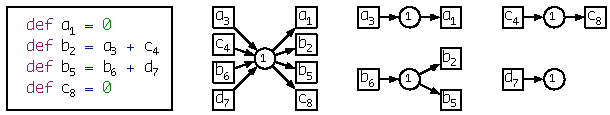
\includegraphics{figures/scope-graphs/global/example.pdf}
\end{boxedminipage}
\vspace*{-\baselineskip}
\caption{Declarations and references in global scope.}
\figurelabel{decs-and-refs}
\end{figure}


\paragraph{Duplicate declarations.}

It is possible for a scope to contain multiple references and/or
declarations with the same name.
For example, scope $1$ in \Figure{decs-and-refs} has two declarations of the
variable \pcfmcode{b}.
While the existence of multiple references is normal, multiple
declarations may give rise to multiple resolutions.
For example, the $\pcfmcode{b}_6$ reference in \Figure{decs-and-refs}
resolves to \emph{each} of the two declarations $\pcfmcode{b}_2$ and
$\pcfmcode{b}_5$.  

Typically, correct programs will not declare the same identifier
at two different locations in the same scope,
although some languages have constructs (e.g. or-patterns in OCaml~\cite{ocamlrefman}) that are most
naturally modeled this way. 
But even when the existence of multiple resolutions implies an erroneous program, 
we want the resolution
calculus to identify \emph{all} these resolutions, since IDEs and other
front-end tools need to be able to represent erroneous programs.
For example, a rename refactoring should support consistent renaming of identifiers, even in
the presence of ambiguities (see \Section{applications}).
The ability of our calculus to describe ambiguous resolutions distinguishes it
from systems, such as nominal logic~\cite{Cheney05a}, that inherently require unambiguous resolution of references. 

\vspace*{-0.5\baselineskip}

\subsection{Lexical Scope}

We model lexical scope by means of the \emph{parent} relation on scopes.
In a well-formed scope graph, each scope has at most one parent and the parent
relation is well-founded.
Formally, the partial function $\P{\_}$ maps a scope $S$ to its \emph{parent}
scope $\P{S}$.
Given a scope graph with parent relation we can define the notion of
\emph{reachable} and \emph{visible} declarations in a scope.

\Figure{lexical} illustrates how the parent relation is used to model common
lexical scope patterns.
Lexical scoping is typically presented through nested regions in the abstract
syntax tree, as illustrated by the nested boxes in \Figure{lexical}.
Expressions in inner boxes may refer to declarations in surrounding boxes, but
not vice versa.
Each of the scopes in the program is mapped to a scope (circle) in the scope
graph.
The three scopes correspond to the global scope, the scope for \pcfmcode{fix
f}$_2$, and the scope for \pcfmcode{fun n}$_3$.
The edges from scopes to scopes correspond to the parent relation.
The resolution paths on the right of \Figure{lexical} illustrate the consequences
of the encoding.
From reference \pcfmcode{f}$_6$ both declarations \pcfmcode{f}$_1$ and
\pcfmcode{f}$_2$ are \emph{reachable}, but from reference \pcfmcode{f}$_9$ only
declaration \pcfmcode{f}$_1$ is reachable.
In languages with lexical scoping, the redeclaration of
a variable inside a nested region typically \emph{hides} the outer
declaration.
Thus, the duplicate declaration of variable \pcfmcode{f} does not indicate
a program error in this situation
because only \pcfmcode{f}$_2$ is \emph{visible} from the scope of
\pcfmcode{f}$_6$.


\begin{figure}[t]
\begin{boxedminipage}{\hsize}
\centering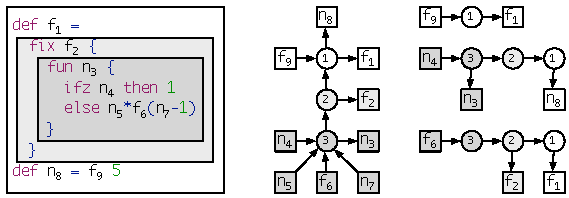
\includegraphics{figures/scope-graphs/lexical/example.pdf}
\end{boxedminipage}
\vspace*{-\baselineskip}
\caption{Lexical scoping modeled by edges between scopes in the scope
graph with example program, scope graph, and reachability paths for
references.}
\figurelabel{lexical}
\end{figure}


\paragraph{Reachability.}

The first step towards a full resolution calculus is to take into account
reachability. We redefine rule $(X_0)$ as follows: 

\begin{center}
	\infrule{X_1}{
		{\ri{x}{i}} \in \R{S_1}
        \tab
        p : S_1 \medge S_2
        \tab
  	    {\di{x}{j}} \in \D{S_2}
	}{
		p : \ri{x}{i} \resolveau \di{x}{j}
	}
\end{center}
	
\noindent
That is, $\ri{x}{i}$ in scope $S_1$ can be resolved to $\di{x}{j}$ in scope $S_2$, if
$S_2$ is \emph{reachable} from $S_1$, i.e. if $S_1 \medge S_2$.
Reachability is defined in terms of the parent relation as follows:

\begin{center}	
   \infrulenl{
		\P{S_1} = S_2
	}{
		\pstep : S_1 \edge S_2
	}
	\infrulenl{
	}{
		[] : A \medge A
	}
	\infrulenl{
		s : A \edge B
		\tab 
		p : B \medge C
	}{
		s \cdot p : A \medge C
	}
\end{center}

\noindent The parent relation between scopes gives rise to a direct edge $S_1
\edge S_2$ between child and parent scope, and $A \medge B$ is the reflexive, transitive
closure of the direct edge relation. 
In order to reason about the different ways in which a reference can be
resolved, we record the resolution path $p$. 
For example, in \Figure{lexical} reference \pcfmcode{f}$_6$ can be resolved with
path $\pstep$ to declaration \pcfmcode{f}$_2$ and with path
$\pstep\cdot\pstep$ to \pcfmcode{f}$_1$.


\paragraph{Visibility.}

Under lexical scoping, multiple possible resolutions are not problematic, as long as
the declarations reached are not declared in the same scope.
A declaration is \emph{visible} unless it is shadowed by a declaration that is
`closer by'.
To formalize visibility, we first extend reachability of scopes to
\emph{reachability of declarations}:

\display{		
	\infrule{R_2}{
                \di{x}{i} \in \D{S'}
                \tab
                p : S \medge S'
	}{
		p \cdot \dstep{\di{x}{i}} : S \reach \di{x}{i}
	}
}

\noindent
That is, a declaration $\di{x}{i}$ in $S'$ is reachable from scope $S$ ($S \reach
\di{x}{i}$), if scope $S'$ is reachable from $S$.

Given multiple reachable declarations, which one should we prefer? A reachable
declaration $\di{x}{i}$ is \emph{visible} in scope $S$ ($S \resolve \di{x}{i}$) if
there is no other declaration for the same name that is reachable
through a \emph{more specific} path:

\display{
  \infrule{V_2}{
 		p : S \reach \di{x}{i}
    \tab \tab
  	\forall j,p' (
  		 p' : S \reach \di{x}{j} \Rightarrow 
  		 \neg (p' < p)
  	)
  }{
		{p} : S \resolve \di{x}{i}
  }
}

\noindent
where the \emph{specificity ordering} $p' < p$ on paths is defined as


\vspace*{-0.5\baselineskip}

\display{
	\infrulenl{}{
		 \dstep{\_} < \pstep
	}
    \infrulenl{
		s_1 < s_2
	}{ 
		s_1\cdot p_1 < s_2 \cdot p_2
	}
	\infrulenl{
		p_1 < p_2
	}{ 
		s \cdot p_1 < s \cdot p_2
	}
}


\vspace*{-0.5\baselineskip}

\noindent
That is, a path with fewer parent transitions is more specific than a path with more
parent transitions.
This formalizes the notion that a declaration in a ``nearer'' scope shadows a
declaration in a ``farther'' scope.
	
Finally, a reference resolves to a declaration if that declaration is visible
in the scope of the reference.
	
\vspace*{-0.5\baselineskip}

\display{
   \infrule{X_2}{
		\ri{x}{i} \in \R{S}
        \tab
        p : S \resolve \di{x}{j}
	}{
		p : \ri{x}{i} \resolve \di{x}{j}
	}
}

\vspace*{-\baselineskip}

\paragraph{Example.}

In \Figure{lexical} the scope (labeled 3) containing 
reference \pcfmcode{f}$_6$ can reach two declarations for $\pcfmcode{f}$:
$\pstep\cdot\dstep{\di{\pcfmcode{f}}{2}} : S_3 \reach \di{\pcfmcode{f}}{2}$
and
$\pstep\cdot\pstep\cdot\dstep{\di{\pcfmcode{f}}{1}} : S_3 \reach
\di{\pcfmcode{f}}{1}$.
Since the first path is more specific than the second path, only \pcfmcode{f}$_2$ is
visible, i.e. $\pstep\cdot\dstep{\di{\pcfmcode{f}}{2}} : S_3 \resolve
\di{\pcfmcode{f}}{2}$.
Therefore \pcfmcode{f}$_6$ resolves to
\pcfmcode{f}$_2$, i.e. $\pstep\cdot\dstep{\di{\pcfmcode{f}}{2}} :
\ri{\pcfmcode{f}}{6} \resolve \di{\pcfmcode{f}}{2}$. 

\paragraph{Scopes, revisited.}
Now that we have defined the notions of reachability and visibility, we can
give a more precise description of the sense in which scopes ``behave
uniformly'' with respect to resolution.  For every scope $S$:
\begin{itemize}
\item Each declaration in the program is either visible
at every reference in $\R{S}$ or not visible at any reference in $\R{S}$.
\item For each reference in the program, either every declaration in $\D{S}$ is
reachable from that reference, or no declaration in $\D{S}$ is reachable 
from that reference. 
\item Every declaration in $\D{S}$ is visible at every reference in $\R{S}$.
\end{itemize}

\subsection{Imports}
\sectionlabel{imports}

Introducing modules and imports complicates the name binding picture.
Declarations are no longer visible only through the lexical context, but may be
visible through an import as well.
Furthermore, resolving a reference may require first resolving one or more
imports, which may in turn require resolving further imports, and so on. 

We model an \emph{import} by means of a reference $\ri{x}{i}$ in the set of imports
$\I{S}$ of a scope $S$. (Imports are also always references and included
in some $\R{S'}$, but not necessarily in the same scope in which they are
imports.)
We model a \emph{module} by associating a scope $S$ with
a declaration $\dsi{x}{i}{S}$.  
This associated \emph{named scope} (i.e., named by $x$) 
represents the declarations introduced by, and
encapsulated in, the module.
(We write the $:\!\!S$ only in rules where it is required; where we omit
it, the declaration may or may not have an associated scope.)
Thus, \emph{importing} entails resolving the import reference to a declaration
and making the declarations in the scope associated with that declaration
available in the importing scope.

%\paragraph{Applications.}

Note that `module' is not a built-in concept in our framework.
A module is any construct that (1) is named, (2) has an associated scope that
encapsulates declarations, and (3) can be imported into another scope.
Of course, this can be used to model the module systems of languages such as ML. 
But it can be applied to constructs that are not modules at first glance.
For example, a class in Java encapsulates class variables and methods, which are
imported into its subclasses through the `extends' clause. 
Thus, a class plays the role of module and the extends clause that of import.
We discuss further applications in \Section{coverage}.


\begin{figure}[t]
\begin{boxedminipage}{\hsize}
\centering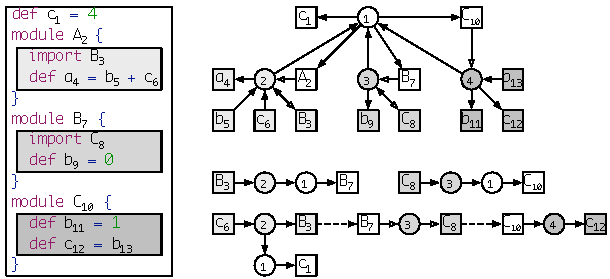
\includegraphics{figures/scope-graphs/imports/imports.pdf}
\end{boxedminipage}
\vspace*{-\baselineskip}
\caption{Modules and imports with example program, scope graph, and reachability
paths for references.}
\figurelabel{imports}
\end{figure}


\paragraph{Reachability.}

To define name resolution in the presence of imports, we first extend the
definition of reachability.
We saw above that the parent relation on scopes induces an edge $S_1 \edge
S_2$ between a scope $S_1$ and its parent scope $S_2$ in the scope graph.
Similarly, an import induces an edge $S_1 \edge S_2$ between a scope $S_1$ and
the scope $S_2$ associated with a declaration imported into $S_1$:

\vspace*{-0.5\baselineskip}

\display{
	\infrule{I_3}{
		\ri{y}{i} \in \I{S_1}  
		\tab
		p : \ri{y}{i} \resolve \dsi{y}{j}{S_2}
	}{
		\istep{\ri{y}{i}}{\dsi{y}{j}{S_2}} : S_1 \edge S_2 
	}
}

\vspace*{-0.5\baselineskip}

\noindent
Note the recursive invocation of the resolution relation on the name of the
imported scope. 

Figure~\figureref{imports} illustrates extensions to scope graphs and paths
to describe imports.
Association of a name to a scope is indicated by an open-headed arrow from the
name declaration box to the scope circle. (For example, scope 2 is associated to
declaration $\pcfmcode{A}_2$.)  An import into a scope is indicated by 
an open-headed arrow from the scope circle to the import name reference box. 
(For example, scope 2 imports the contents of the scope associated to 
the resolution of reference $\pcfmcode{B}_3$; note that 
since $\pcfmcode{B}_3$ is also a reference within scope 2, there is also an ordinary
arrow in the opposite direction, leading to a double-headed arrow in the scope graph.)
Edges in reachability paths representing the resolution of imported
scope names to their definitions are drawn dashed. (For example, reference
$\pcfmcode{B}_3$ resolves to declaration $\pcfmcode{B}_7$, which has associated
scope 3.)  The paths at the bottom right of the figure illustrate that 
the scope (labeled 2) containing reference $\pcfmcode{c}_6$ 
can reach two declarations for $\pcfmcode{c}$: 
$\pstep\cdot\dstep{\di{\pcfmcode{c}}{1}} : S_2 \reach \di{\pcfmcode{c}}{1}$
and $\istep{\ri{\pcfmcode{B}}{3}}{\dsi{\pcfmcode{B}}{7}{S_3}}\cdot
\istep{\ri{\pcfmcode{C}}{8}}{\dsi{\pcfmcode{C}}{10}{S_4}}\cdot
\dstep{\di{\pcfmcode{c}}{12}} : S_2 \reach \di{\pcfmcode{c}}{12}$,
making use of the subsidiary resolutions
$\ri{\pcfmcode{B}}{3} \resolve \di{\pcfmcode{B}}{7}$ and
$\ri{\pcfmcode{C}}{8} \resolve \di{\pcfmcode{C}}{10}$.


\begin{wrapfigure}[22]{r}{2.5cm}
\vspace*{-0.9\baselineskip}
\begin{lstlisting}
def a$_1$ = ...
module A$_2$ {
  def a$_3$ = ... 
  def b$_4$ = ...
}
module C$_5$ {
  import A$_6$
  def b$_7$ = a$_8$
  def c$_9$ = b$_{10}$
}
\end{lstlisting}
\vspace*{-\baselineskip}
\caption{Parent vs Import}
\figurelabel{parent-vs-import}
\smallskip
% \end{wrapfigure}
% \begin{wrapfigure}[12]{r}{2.5cm}
%\vspace*{-1.7\baselineskip}
\begin{lstlisting}
def a$_1$ = ...
module B$_2$ {
}
module C$_3$ {
  def a$_4$ = ...
  module D$_5$ {
    import B$_6$
    def e$_7$ = a$_8$
  }
}
\end{lstlisting}
\vspace*{-\baselineskip}
\caption{Parent of import}
\figurelabel{parent-of-import}
\end{wrapfigure} 

\paragraph{Visibility.}

Imports cause new kinds of ambiguities in resolution paths, which require
extension of the visibility policy.

The first issue is illustrated by \Figure{parent-vs-import}.
In the scope of reference \pcfmcode{b}$_{10}$ we can reach declaration
\pcfmcode{b}$_7$ with path $\dstep{\di{\pcfmcode{b}}{7}}$ and
declaration \pcfmcode{b}$_4$ with path
$\istep{\ri{A}{6}}{\dsi{A}{2}{S_A}}\cdot\dstep{\di{\pcfmcode{b}}{4}}$
(where $S_A$ is the scope named by declaration $A_2$).
We resolve this conflict by extending the specificity order with the rule
$\dstep{\_} < \istep{\_}{\_}$.
That is, local declarations override imported declarations.
Similarly, in the scope of reference \pcfmcode{a}$_8$ we can reach declaration
\pcfmcode{a}$_1$ with path $\pstep\cdot\dstep{\di{\pcfmcode{a}}{1}}$ and
declaration \pcfmcode{a}$_3$ with path
$\istep{\ri{A}{6}}{\dsi{A}{2}{S_A}}\cdot\dstep{\di{\pcfmcode{a}}{3}}$. 
We resolve this conflict by extending the specificity order with the rule
$\istep{\_}{\_} < \pstep$.
That is, resolution through imports is preferred over resolution through
parents. 
In other words, declarations in imported modules override declarations in
lexical parents.




The next issue is illustrated in \Figure{parent-of-import}. 
In the scope of reference \pcfmcode{a}$_8$ we can reach declaration
\pcfmcode{a}$_4$ with path $\pstep\cdot\dstep{\di{\pcfmcode{a}}{4}}$ and
declaration \pcfmcode{a}$_1$ with path $\pstep\cdot\pstep\cdot\dstep{\di{\pcfmcode{a}}{1}}$.
The specificity ordering guarantees that only the first of these is visible, giving
the resolution we expect.  However, with the rules as stated so far, there
is another way to reach \pcfmcode{a}$_1$, via the path
$\istep{\ri{\pcfmcode{B}}{6}}{\dsi{\pcfmcode{B}}{2}{S_B}}\cdot
\pstep\cdot\dstep{\di{\pcfmcode{a}}{1}}$.
That is, we first import module \pcfmcode{B}, and then go to its lexical 
parent, where we find the declaration.  In other words,
when importing a module, we 
import not just its declarations, but all declarations in its lexical context.
This behavior seems undesirable; to our knowledge, no real languages exhibit it. 
To rule out such resolutions, we define a well-formedness predicate $\WF(p)$
that requires paths $p$ to be of the form $\pstep^* \cdot \istep{\_}{\_}^*$, 
i.e. forbidding the use of parent steps after one or more import
steps. We use this predicate to restrict the reachable declarations relation by
only considering scopes reachable through a well-formed path:

\display{
	\infrule{R_3}{
		\di{x}{i} \in \D{S'}
		\tab
		p : S \medge S'
		\tab 
		\WF(p)
	}{
		p \cdot \dstep{\di{x}{i}} : S \reach \di{x}{i}
	}
}	

\noindent
The complete definition of well-formed paths and specificity order on paths is
given in \Figure{order}.
In \Section{extensions} we discuss how alternative visibility policies can be
defined by just changing the well-formedness predicate and specificity order.

\begin{figure}[t]
\begin{boxedminipage}{\hsize}
$$
\inferrule*{  
  \inferrule*{
    \inferrule*{
      \dsi{A}{2}{S_{A_2}} \in \D{S_{A_1}} 
      \tab
      \inferrule*{
        \ri{A}{4} \in \I{S_{root}}
        \tab
        \inferrule*{
          \ri{A}{4} \in \R{S_{root}}
          \\
          \dsi{A}{1}{S_{A_1}} \in \D{S_{root}}
        }{
          \ri{A}{4} \resolve \dsi{A}{1}{S_{A_1}}
        }
      }{
        S_{root} \edge S_{A_1} \tab (*)
      }
    }{
      S_{root} \reach \dsi{A}{2}{S_{A_2}}  
    }
  }{
    \ri{A}{4} \in \R{S_{root}}
    \tab 
    S_{root} \resolve \dsi{A}{2}{S_{A_2}}
  }
}{
\ri{A}{4} \resolve \dsi{A}{2}{S_{A_2}}
}
$$
\end{boxedminipage}
\vspace*{-\baselineskip}
\caption{Derivation for $\ri{A}{4} \resolve \dsi{A}{2}{S_{A_2}}$ in a calculus without import tracking.}
\figurelabel{self-import-derivation}
\end{figure}

\begin{wrapfigure}[20]{r}{2.6cm}
\vspace*{-.7\baselineskip}
\begin{lstlisting}
module A$_1$ { 
  module A$_2$ { 
    def a$_3$ = ...
  } 
}
import A$_4$
def b$_5$ = a$_6$
\end{lstlisting}
\vspace*{-\baselineskip}
\caption{Self import}
\figurelabel{self-import}
\medskip

% \end{wrapfigure}
% \begin{wrapfigure}[12]{r}{2.5cm}
%\vspace*{-\baselineskip}
\begin{lstlisting}
module A$_1$ {
  module B$_2$ { 
    def x$_3$ = 1 
  }
}
module B$_4$ {
  module A$_5$ { 
    def y$_6$ = 2 
  }
}
module C$_7$ {
  import A$_8$
  import B$_9$
  def z$_{10}$ = x$_{11}$ 
          + y$_{12}$
}
\end{lstlisting}
\vspace*{-\baselineskip}
\caption{Anomalous resolution}
\figurelabel{anomalous}
\end{wrapfigure}


\paragraph{Seen imports.}

Consider the example in \Figure{self-import}. 
Is declaration \pcfmcode{a}$_3$ reachable in the scope of reference
\pcfmcode{a}$_6$?
This reduces to the question whether the import of \pcfmcode{A}$_4$ can resolve to
module \pcfmcode{A}$_2$.
Surprisingly, it can, in the calculus as discussed so far, as shown by the
derivation in \Figure{self-import-derivation} (which takes a few shortcuts).
The conclusion of the derivation is that 
$\ri{A}{4} \resolve \dsi{A}{2}{S_{A_2}}$.
This conclusion is obtained by \emph{using the import at \pcfmcode{A}$_4$}
to conclude at step (*) that $S_{root} \edge S_{A_1}$, i.e. that the body of
module \pcfmcode{A}$_1$ is reachable!
In other words, the import of \pcfmcode{A}$_4$ is used in its own
resolution.  Intuitively, this is nonsensical.

To rule out this kind of behavior we extend the calculus to keep track of the
set of \emph{seen imports} $\seeni$ using judgements of the form 
$\seeni \vdash p : \ri{x}{i} \resolve \di{x}{j}$. 
We need to extend all rules to pass the set $\seeni$, but only the rules
for resolution and import are truly affected:

%\vspace*{-.5\baselineskip}

\display{
	\infrule{X}{
		\ri{x}{i} \in \R{S}
        \tab
        \{ \ri{x}{i} \} \cup \seeni \vdash p : S \resolve \di{x}{j}
	}{
		\seeni \vdash p : \ri{x}{i} \resolve \di{x}{j}
	}
}

\vspace*{-1.5\baselineskip}

\display{
	\infrule{I}{
		\ri{y}{i} \in \I{S_1}\setminus\seeni  
		\tab
		\seeni \vdash p : \ri{y}{i} \resolve \dsi{y}{j}{S_2}
	}{
		\seeni \vdash \istep{\ri{y}{i}}{\dsi{y}{j}{S_2}} : S_1 \edge S_2 
	}
}

%\vspace*{-0.5\baselineskip}


With this final ingredient, we reach the full calculus in \Figure{rescalc}.
It is not hard to see that the resolution relation is well-founded. The only
recursive invocation (via the $I$ rule) uses a strictly larger set $\seeni$
of seen imports (via the $X$ rule); since the set $\R{G}$ is finite, $\seeni$ cannot
grow indefinitely.

\paragraph{Anomalies.}

Although the calculus produces the desired resolutions for a wide variety
of real language constructs, its behavior can be surprising on corner cases.
Even with the ``seen imports'' mechanism, it is still possible for
a single derivation to resolve a given import in two different ways, leading to 
unintuitive results.  For example, in the program in \Figure{anomalous},
\pcfmcode{x}$_{11}$ can resolve to \pcfmcode{x}$_3$ and
\pcfmcode{y}$_{12}$ can resolve to \pcfmcode{y}$_6$. (Derivations left as an exercise
to the curious reader!)  
In our experience, phenomena like this occur only in the presence of
mutually-recursive imports; to our knowledge, no real language has these
(perhaps for good reason).  We defer deeper exploration of these anomalies
to future work.


%%%%%%%%%%%%%%%%%%%%%%%%%%%%%%%%%%%%%%%%%%%%%%%%%%
\endinput
	  
\paragraph{Cyclic Import Dependencies}

\begin{lstlisting}
module A { import B }
module B { import A }
\end{lstlisting}

\begin{lstlisting}
module A {
   module B {}
}
module B {
   module A {}
}
module M {
   import C;
   import D;   
   module C { import A };
   module D { import B }
} 
\end{lstlisting}

The resolution of {\tt A} can use {\tt import B} through {\tt import D} and the resolution of {\tt B} can use {\tt import A} through {\tt import C}.
Thus with seen imports both imports resolve to the innermost modules.
The following program also has the same behavior:

\begin{lstlisting}
module A {
   module B {}
}
module B {
   module A {}
}
module M {
   import C.D; 
   module C {     
      import A 
      module D { 
         import B }
      }
   }
} 
\end{lstlisting}




\paragraph{}


Notice that the identifier of an import can have a different enclosing scope than the
scope for which it is an import. 

That is, the implication $x^p \in \I{S}
\Rightarrow x^p \in \R{S}$ does \emph{not} hold. 
For example, in \Figure{includes}, the identifier $B_1$ is a
reference in scope 3, but an import in scope 2.

\subsection{Errors in Resolved Scope Graph}

\parindent0pt
\parskip0.5\baselineskip
\TODO{remove parindent/parskip commands}
	
problems in programs that lead to errors in scope graph

how this would be presented in the IDE

unresolved reference

ambiguous / conflicting resolution

quick fixing




\subsection{Construction of Scope Graph}

\TODO{algorithm for construction of scope graph for LM programs}


A scope often corresponds to a node in the AST, but this is not necessarily the
case. 

how one arrives at the set of program points 

The very challenge of formulating a theory of name resolution is to describe the
rules

a scope is smaller than a traditional scope



Languages use scoping constructs to restrict the visibility of names.
A name declared in a scope is not visible outside that scope.





